\section{Bitcoin}
\label{sec:bitcoin}

Am 01. November 2008 veröffentlichte "`Satoshi Nakamoto"' über eine Mailingliste \cite{bitcoinmailinglist} ein Paper \cite{bitcoinpaper}, in dem
er Bitcoin als digitale Währung vorstellte. Obwohl bis heute nicht bekannt ist, wer sich hinter diesem Namen verbirgt, hat sich Bitcoin seit der
Lösung des ersten "`Blocks"' am 03. Januar 2009 \cite{bitcoinblock0} weit verbreitet. Wie ein Block gelöst wird, ist der einzige Aspekt der für
diese Arbeit eine Rolle spielt und wird im folgenden erläutert.

Bitcoin basiert auf einer Kette von Blöcken (Blockchain). Ein Block dient dazu, Transaktionen zwischen Benutzern zu bestätigen, die seit der Lösung
des letzten Blocks durchgeführt wurden. Da auch der letzte Block in die Lösung mit einbezogen wird, wird die gesamte Kette erneut bestätigt.
Für die Lösung eines Blocks wird die Hashfunktion SHA256 \ref{chp:sha256} genutzt. Neben dem letzte Block, den aktuellen Transaktionen und einiger
weiterer Daten fließt insbesondere eine Nonce als Eingabe in die Hashfunktion ein die frei gewählt werden kann um den Block zu lösen. Gelöst ist ein
Block dann, wenn durch die Wahl der Nonce und zweimaliger Anwendung von SHA256 ein Hash erzeugt wird, der mit entsprechend vielen Nullen beginnt
(siehe Abbildung \ref{fig:bitcoin}). Je mehr Nullen gefordert sind, desto schwieriger wird diese Aufgabe.

\begin{figure}[!h]
  \centering
  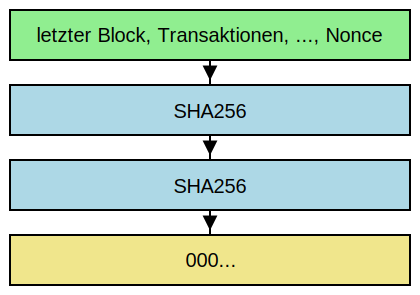
\includegraphics[scale=0.4]{images/bitcoin}
  \caption{Schematische Darstellung einer Blockberechnung}
  \label{fig:bitcoin}
\end{figure}

Da eine Hashfunktion eine Einwegfunktion ist, kann eine gültige Nonce nur durch ausprobieren aller möglichen Werte gefunden werden. Als Motivation
für diesen Prozess Rechenleistung zu investieren, werden derzeit 12 Bitcoins an den Benutzer ausgeschüttet, der als erster eine gültige Nonce liefert.



